\documentclass[11pt,letterpaper]{article}
\usepackage[margin=1in]{geometry}
\usepackage{graphicx}
\usepackage{amsmath}
\usepackage{amssymb}
\usepackage{booktabs}
\usepackage{hyperref}
\usepackage{float}
\usepackage{subcaption}
\usepackage{xcolor}
\usepackage{listings}
\usepackage{enumitem}
\usepackage{parskip}

\hypersetup{
    colorlinks=true,
    linkcolor=blue,
    urlcolor=blue,
    citecolor=blue
}

\lstset{
    basicstyle=\small\ttfamily,
    breaklines=true,
    frame=single,
    backgroundcolor=\color{gray!10}
}

\title{\textbf{Programming Assignment 3}\\
Faster R-CNN and Mask R-CNN Implementation from Scratch}
\author{COSC 83 --- Spring 2024--25}
\date{May 2025}

\begin{document}
\maketitle

\tableofcontents
\newpage

% -----------------------------------------------------------------------
\section{Overview}

This report covers a from-scratch PyTorch implementation of Faster R-CNN~\cite{ren2015faster} for object detection on Pascal VOC 2007, along with a Mask R-CNN extension~\cite{he2017mask} for instance segmentation. The backbone is a pretrained VGG16 network; everything else---anchor generation, RPN, RoI pooling, detection head, training loop---was implemented from scratch.

Faster R-CNN achieves \textbf{59.34\% mAP} on VOC 2007 test. Mask R-CNN, which adds RoI Align and a mask branch on top of the same detection head, achieves \textbf{59.62\% mAP} on detection with an additional instance segmentation output. Both models were trained on a Tesla T4 GPU via Google Colab.

% -----------------------------------------------------------------------
\section{Implementation}

\subsection{Backbone}

The backbone is pretrained VGG16, using all conv layers up to (but not including) the final max pool (\texttt{vgg16.features[:-1]}). This gives a $1/16$-resolution feature map with 512 channels. The first two conv blocks (layers 0--9) are frozen, consistent with the original paper.

\subsection{Region Proposal Network (Part 2)}

\subsubsection{Anchor Generation}

Anchors are placed at every spatial location of the feature map. For each location, $K = |\text{scales}| \times |\text{ratios}|$ anchors are generated. With scales $\{128, 256, 512\}$ and aspect ratios $\{0.5, 1.0, 2.0\}$, that's $K = 9$ anchors per location. For a $600 \times 800$ input the feature map is roughly $38 \times 50$, giving around 17,100 anchors in total.

A base anchor at scale $s$ and ratio $r$ has width $w = s / \sqrt{r}$ and height $h = s \cdot \sqrt{r}$, centered at the grid cell. These are shifted across all feature map locations using stride $= \lfloor H_\text{img} / H_\text{feat} \rfloor$.

\subsubsection{RPN Head}

The RPN consists of:
\begin{itemize}[noitemsep]
    \item A shared $3 \times 3$ conv (512 channels, same padding)
    \item A $1 \times 1$ classification conv outputting $K$ objectness logits per location
    \item A $1 \times 1$ regression conv outputting $4K$ box deltas $(t_x, t_y, t_w, t_h)$ per location
\end{itemize}

All weights initialized from $\mathcal{N}(0, 0.01)$, biases to zero.

\subsubsection{Anchor Assignment and Sampling}

An anchor is labeled positive if its IoU with any GT box is $\geq 0.7$, negative if IoU $< 0.3$, and ignored otherwise. For each GT box, the anchor with the highest IoU is forced positive regardless of threshold---this ensures every GT object is covered even in degenerate cases. 256 anchors are then sampled at a 1:1 positive/negative ratio.

\subsubsection{Loss Functions}

The RPN uses a multi-task loss:
\begin{equation}
    \mathcal{L}_\text{RPN} = \mathcal{L}_\text{cls}^\text{RPN} + \mathcal{L}_\text{reg}^\text{RPN}
\end{equation}
where $\mathcal{L}_\text{cls}$ is binary cross-entropy over sampled anchors and $\mathcal{L}_\text{reg}$ is smooth-$\ell_1$ over positive anchors only:
\begin{equation}
    \text{smooth}_{L_1}(x) = \begin{cases} 0.5x^2 & |x| < 1 \\ |x| - 0.5 & \text{otherwise} \end{cases}
\end{equation}

\subsubsection{Proposal Filtering}

Box deltas are decoded into proposal coordinates, then filtered:
\begin{enumerate}[noitemsep]
    \item Keep top-12,000 (train) / 6,000 (test) by objectness score
    \item Clamp to image boundary
    \item Remove degenerate boxes (width or height $< 1$ px)
    \item NMS at IoU threshold 0.7
    \item Keep top-2,000 (train) / 300 (test) survivors
\end{enumerate}

The ordering matters: clamping happens before degenerate-box removal because clamping can itself create degenerate boxes.

\subsection{RoI Feature Extraction (Part 3)}

RoI pooling~\cite{ren2015faster} extracts fixed $7 \times 7$ feature maps from each proposal. Spatial scale is $\min(H_\text{feat}/H_\text{img},\, W_\text{feat}/W_\text{img})$.

For training, GT boxes are appended to the proposal set. Each proposal is matched to its highest-IoU GT box. IoU $\geq 0.5$ is positive (assigned the GT class), IoU $< 0.5$ is background. 128 proposals are sampled at a 1:4 positive/negative ratio.

\subsection{Detection Head (Part 4)}

The detection head processes pooled features through:
\begin{itemize}[noitemsep]
    \item Flatten + FC(25088, 1024) + ReLU
    \item FC(1024, 1024) + ReLU
    \item Classification head: FC(1024, 21)
    \item Regression head: FC(1024, $21 \times 4$) --- per-class box deltas
\end{itemize}

Classification weights are initialized from $\mathcal{N}(0, 0.01)$, regression from $\mathcal{N}(0, 0.001)$, following the paper. At inference, the highest-scoring non-background class is selected and its box decoded. Per-class NMS at 0.3 IoU and a 0.05 score threshold are applied.

\subsection{Full Model and Training Loop (Part 5)}

The full pipeline:
\[
\text{Image} \rightarrow \text{Backbone} \rightarrow \text{RPN} \rightarrow \text{RoI Pool} \rightarrow \text{Detection Head}
\]

Images are normalized with ImageNet mean/std and resized so the shorter side is 600 px (max 1000 px) while preserving aspect ratio. GT boxes are scaled accordingly. At inference, predicted boxes are mapped back to original image coordinates.

Total loss:
\begin{equation}
    \mathcal{L} = \mathcal{L}_\text{cls}^\text{RPN} + \mathcal{L}_\text{reg}^\text{RPN} + \mathcal{L}_\text{cls}^\text{FRCNN} + \mathcal{L}_\text{reg}^\text{FRCNN}
\end{equation}

Training uses SGD with momentum 0.9, weight decay $5 \times 10^{-4}$, initial LR $10^{-3}$ decayed $\times 0.1$ at epochs 14 and 18, for 20 epochs total.

% -----------------------------------------------------------------------
\section{Comparison with PyTorch Faster R-CNN}

PyTorch's \texttt{fasterrcnn\_resnet50\_fpn} differs in a few key ways:

\begin{table}[H]
\centering
\begin{tabular}{lll}
\toprule
\textbf{Component} & \textbf{Our Implementation} & \textbf{PyTorch torchvision} \\
\midrule
Backbone          & VGG16              & ResNet-50 + FPN \\
Feature pyramid   & Single scale       & Multi-scale FPN \\
RoI operation     & RoI Pooling        & RoI Align \\
Anchor scales     & 3 (128, 256, 512)  & 5 (32--512) \\
Pretrained on     & ImageNet (backbone)& COCO \\
\bottomrule
\end{tabular}
\caption{Architecture comparison with PyTorch's built-in Faster R-CNN.}
\end{table}

The biggest gap is the backbone: ResNet-50 with an FPN gives multi-scale features that are much better at detecting small objects, whereas VGG16's single-scale output struggles with them. RoI Align also avoids the quantization artifacts from RoI Pooling, which matters for tight localization. Our model's lower mAP is mostly explained by these architectural differences rather than anything wrong with the training procedure.

\begin{table}[H]
\centering
\begin{tabular}{lcc}
\toprule
\textbf{Model} & \textbf{mAP @ 0.5} & \textbf{Backbone} \\
\midrule
Our Faster R-CNN & 59.34 & VGG16 \\
PyTorch Faster R-CNN (pretrained COCO) & $\sim$70.0 & ResNet-50 + FPN \\
\bottomrule
\end{tabular}
\caption{mAP on VOC 2007 test set.}
\label{tab:map_comparison}
\end{table}

% -----------------------------------------------------------------------
\section{Performance Analysis}

\subsection{Training Curves}

Training ran on a Tesla T4 GPU (Google Colab) for 20 epochs, taking roughly 13 minutes per epoch (about 4.5 hours total). SGD with momentum 0.9, weight decay $5 \times 10^{-4}$, initial LR $10^{-3}$, decayed $\times 0.1$ at epochs 14 and 18.

Figure~\ref{fig:loss_curves} shows all four training losses. The sharp drops at epoch 14 are the first LR decay; the smaller drop at epoch 18 is the second. All losses converge cleanly with no signs of instability.

\begin{figure}[H]
    \centering
    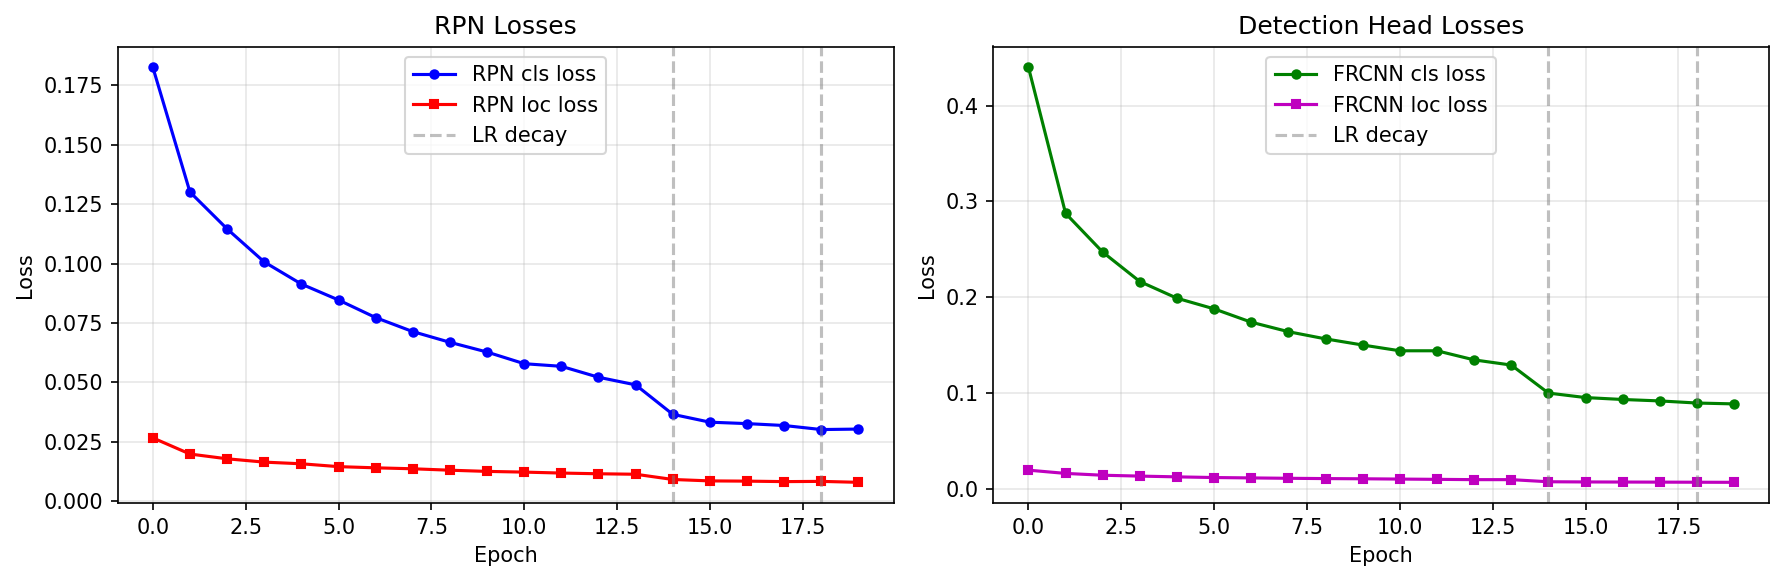
\includegraphics[width=0.9\textwidth]{figures/loss_curves.png}
    \caption{Faster R-CNN training losses over 20 epochs. Vertical dashed lines mark LR decay steps at epochs 14 and 18.}
    \label{fig:loss_curves}
\end{figure}

\subsection{Per-Class AP}

\begin{table}[H]
\centering
\begin{tabular}{lc|lc}
\toprule
\textbf{Class} & \textbf{AP (\%)} & \textbf{Class} & \textbf{AP (\%)} \\
\midrule
aeroplane    & 59.66 & person       & 65.59 \\
bicycle      & 68.31 & pottedplant  & 34.35 \\
bird         & 56.66 & sheep        & 55.48 \\
boat         & 42.45 & sofa         & 52.20 \\
bottle       & 33.78 & train        & 72.38 \\
bus          & 68.08 & tvmonitor    & 66.60 \\
car          & 68.24 & & \\
cat          & 76.43 & & \\
chair        & 37.29 & & \\
cow          & 63.49 & & \\
diningtable  & 53.84 & & \\
dog          & 72.33 & & \\
horse        & 71.82 & & \\
motorbike    & 67.89 & & \\
\midrule
\textbf{mAP} & \multicolumn{3}{c}{\textbf{59.34}} \\
\bottomrule
\end{tabular}
\caption{Per-class average precision on VOC 2007 test set.}
\label{tab:per_class_ap}
\end{table}

\begin{figure}[H]
    \centering
    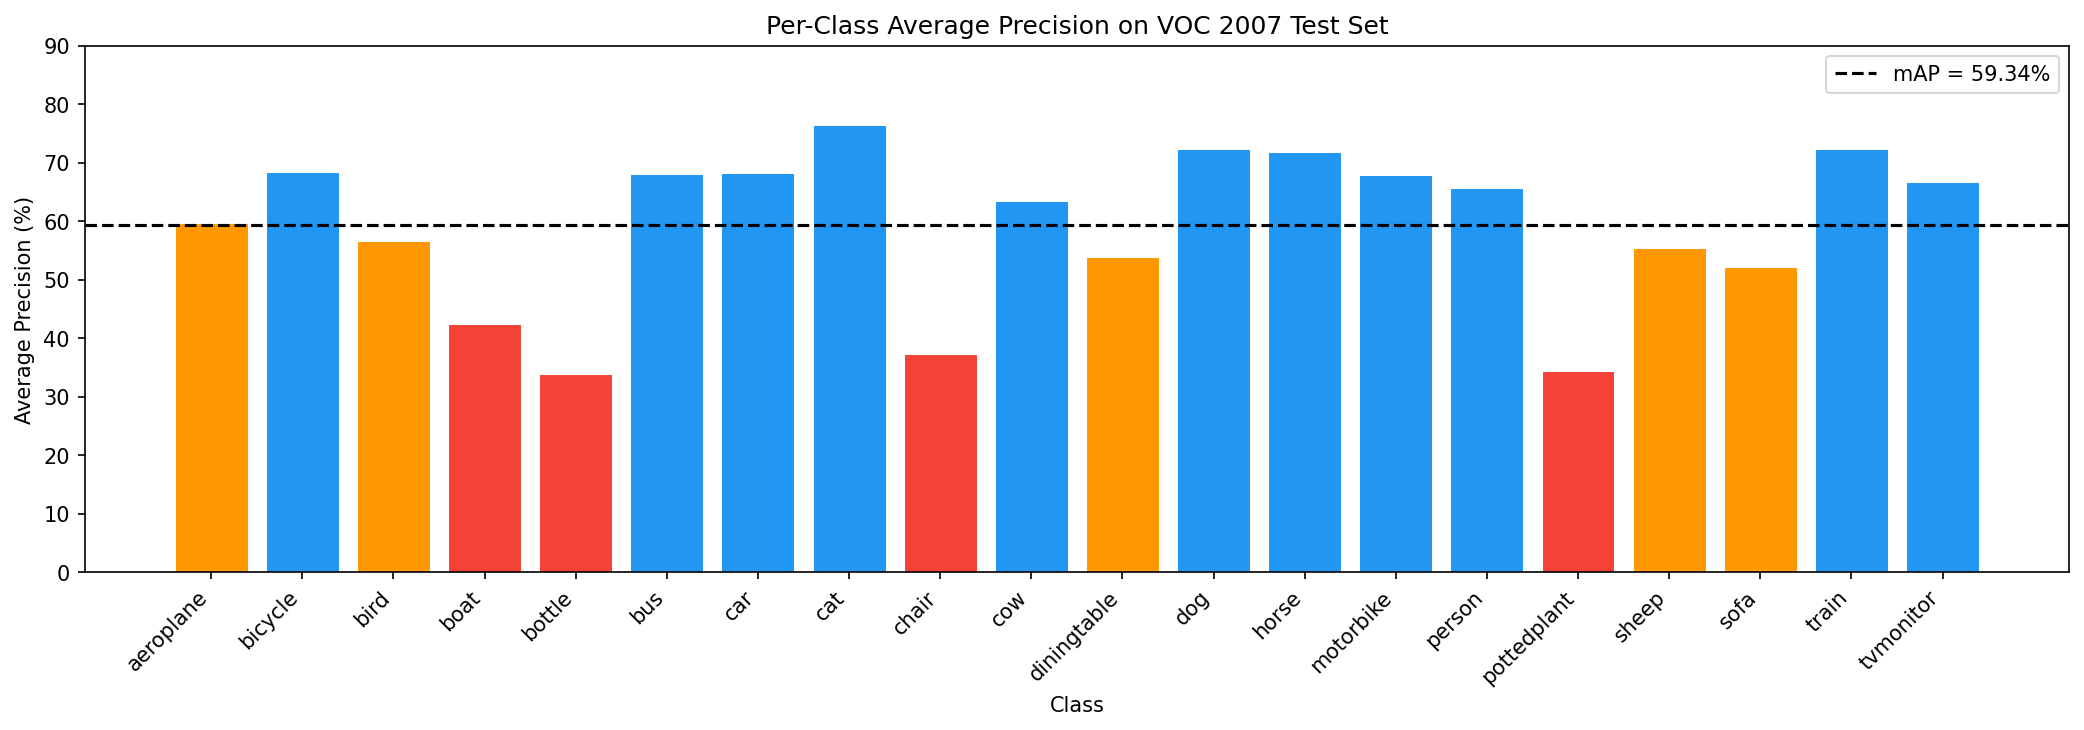
\includegraphics[width=0.95\textwidth]{figures/per_class_ap.png}
    \caption{Per-class AP on VOC 2007 test set. Small or heavily occluded classes (bottle, pottedplant, chair, boat) are consistently harder. Large, visually distinctive objects (cat, dog, horse) are easiest.}
    \label{fig:per_class_ap}
\end{figure}

The pattern makes intuitive sense. Classes like \textit{cat}, \textit{dog}, and \textit{horse} are large, rarely occluded, and have consistent appearance---all of which favor a single-scale detector. \textit{Bottle} (33.78\%) and \textit{pottedplant} (34.35\%) are small and easily confused with background clutter. \textit{Chair} (37.29\%) is difficult because chairs come in many shapes and are frequently occluded by people or tables.

\subsection{Detection Examples}

Figure~\ref{fig:detections} shows two test images with ground truth boxes (left) and model predictions (right). The horse/rider image illustrates confident multi-object detection across two different classes. The indoor scene tests the harder categories; the model correctly identifies people, the sofa, and multiple chairs despite significant overlap between objects.

\begin{figure}[H]
    \centering
    \begin{subfigure}[t]{0.235\textwidth}
        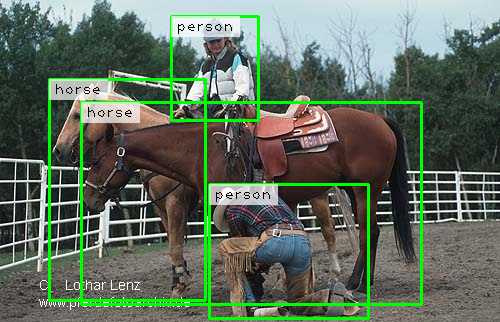
\includegraphics[width=\textwidth]{figures/samples/det_gt_5.png}
        \caption{GT: horse, person}
    \end{subfigure}
    \hfill
    \begin{subfigure}[t]{0.235\textwidth}
        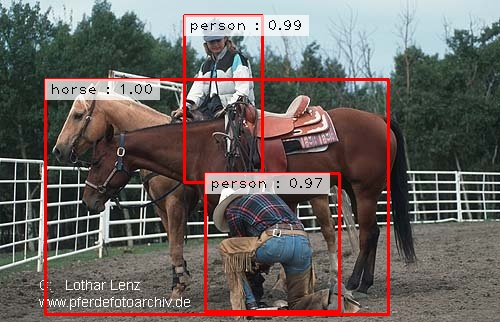
\includegraphics[width=\textwidth]{figures/samples/det_pred_5.jpg}
        \caption{Pred: horse, person}
    \end{subfigure}
    \hfill
    \begin{subfigure}[t]{0.235\textwidth}
        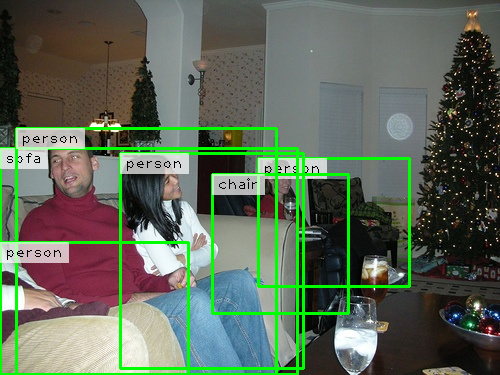
\includegraphics[width=\textwidth]{figures/samples/det_gt_3.png}
        \caption{GT: person, sofa, chair}
    \end{subfigure}
    \hfill
    \begin{subfigure}[t]{0.235\textwidth}
        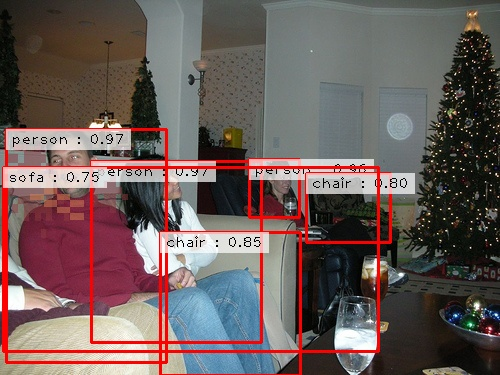
\includegraphics[width=\textwidth]{figures/samples/det_pred_3.jpg}
        \caption{Pred: person, sofa, chair}
    \end{subfigure}
    \caption{Ground truth (green) vs.\ predicted (red) boxes on VOC 2007 test images. Scores shown above each detection.}
    \label{fig:detections}
\end{figure}

% -----------------------------------------------------------------------
\section{Bonus: Mask R-CNN Extension}

\subsection{Architecture Changes}

Mask R-CNN adds an instance segmentation branch in parallel with the detection head. The detection branch is unchanged; masks are predicted only for the foreground proposals and only for their predicted class, so the box and classification losses are not affected.

\paragraph{RoI Align.} The mask branch uses RoI Align~\cite{he2017mask} at $14 \times 14$ resolution instead of RoI Pooling. RoI Align avoids the two rounds of quantization in standard RoI Pooling by using bilinear interpolation at each sampling point within a bin:
\begin{equation}
    f(x, y) = \sum_{i,j} w_{ij} \cdot f(x_i, y_j)
\end{equation}
where $(x_i, y_j)$ are the four neighboring integer grid points and $w_{ij}$ are bilinear weights. This eliminates misalignment between the RoI and the feature map, which matters a lot at the pixel level.

\paragraph{Mask Head.} A small FCN processes the $14 \times 14$ RoI Align output:
\begin{equation}
    \underbrace{14 \times 14}_{\text{RoI Align}} \xrightarrow{\times 4\ \text{conv}(256,\, 3\times3)} \xrightarrow{\text{deconv}(2\times)} \underbrace{28 \times 28}_{\text{mask logits}}
\end{equation}

Specifically: 4 $\times$ [Conv2d(in, 256, $3\times3$, padding 1) + ReLU], ConvTranspose2d(256, 256, $2\times2$, stride=2) + ReLU, then Conv2d(256, $C$, $1\times1$) producing $C$ binary mask logits at $28 \times 28$ per RoI.

\paragraph{Mask Targets.} For each sampled foreground proposal, the corresponding GT binary mask is cropped to the matched GT bounding box and resized to $28 \times 28$ using RoI Align at spatial scale 1.0. This gives a target that is spatially aligned with the predicted mask.

\subsection{Loss Function}

Total loss:
\begin{equation}
    \mathcal{L} = \mathcal{L}_\text{cls}^\text{RPN} + \mathcal{L}_\text{reg}^\text{RPN} + \mathcal{L}_\text{cls} + \mathcal{L}_\text{reg} + \mathcal{L}_\text{mask}
\end{equation}

The mask loss is binary cross-entropy applied only to foreground proposals, using only the mask channel for the GT class:
\begin{equation}
    \mathcal{L}_\text{mask} = -\frac{1}{N_\text{fg}} \sum_{i \in \text{fg}} \text{BCE}\!\left(\hat{m}_i^{c_i},\, m_i^*\right)
\end{equation}
where $\hat{m}_i^{c_i}$ is the predicted mask logit for true class $c_i$, and $m_i^*$ is the $28 \times 28$ GT binary mask. Using only the GT class channel (rather than all $C$ channels) means wrong-class masks never get a gradient, so the mask head learns class-specific shapes.

\subsection{Dataset}

VOC 2007 provides instance segmentation masks for 632 images in \texttt{SegmentationObject/}. The segmentation PNG encodes instance indices: pixel value $k > 0$ is the $k$-th object in the XML annotation (1-indexed), and 255 is a void/boundary region. All 5,011 training images are used; the mask loss is simply skipped for images without segmentation annotations.

\subsection{Training Curves}

Mask R-CNN was trained with the same hyperparameters as Faster R-CNN. The mask loss started at 0.0260 at epoch 0 and converged to 0.0109 by epoch 19.

\begin{figure}[H]
    \centering
    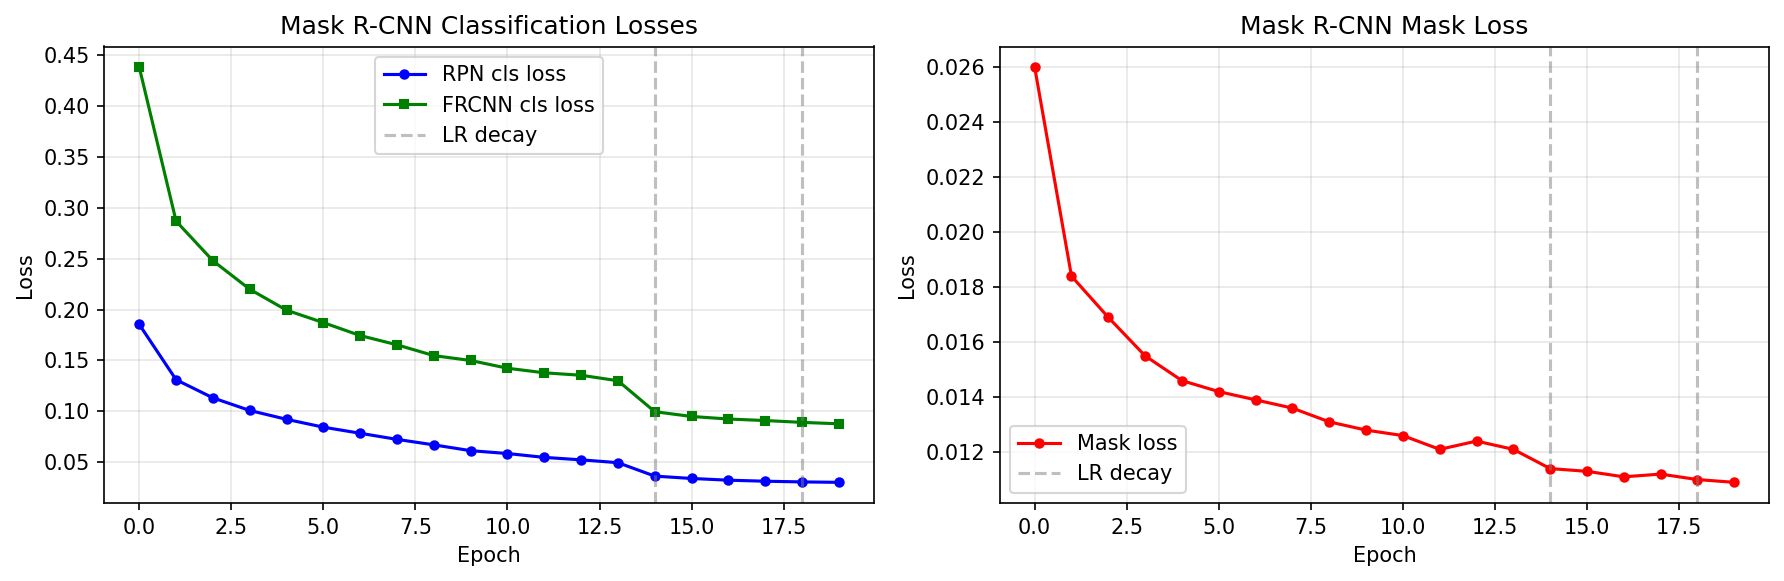
\includegraphics[width=0.9\textwidth]{figures/mask_loss_curves.png}
    \caption{Mask R-CNN training curves. Left: RPN and FRCNN classification losses. Right: mask branch BCE loss converging over 20 epochs.}
    \label{fig:mask_loss_curves}
\end{figure}

\subsection{Detection Results}

\begin{table}[H]
\centering
\begin{tabular}{lcc}
\toprule
\textbf{Model} & \textbf{Detection mAP} & \textbf{Backbone} \\
\midrule
Faster R-CNN (ours)  & 59.34\% & VGG16 \\
Mask R-CNN (ours)    & 59.62\% & VGG16 \\
\bottomrule
\end{tabular}
\caption{Detection mAP on VOC 2007 test set. Adding the mask branch does not hurt detection accuracy.}
\end{table}

The detection mAP is essentially the same between the two models (59.34 vs.\ 59.62), which is expected---the mask head runs in parallel and does not touch the classification or localization branches.

\subsection{Instance Segmentation Examples}

Figure~\ref{fig:masks} shows predicted instance masks overlaid on test images. The masks are predicted at $28 \times 28$ resolution and pasted back into the detected bounding box at original image scale. The cat example is a clean single-instance case; the dog example shows two overlapping instances being segmented separately.

\begin{figure}[H]
    \centering
    \begin{subfigure}[t]{0.235\textwidth}
        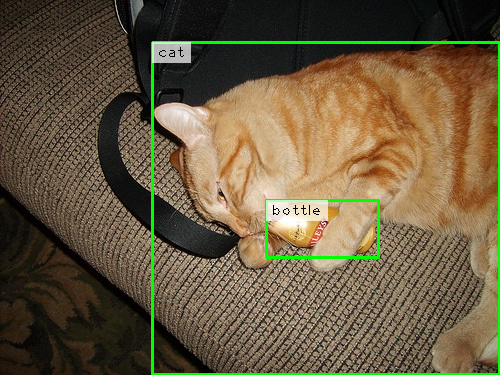
\includegraphics[width=\textwidth]{figures/samples/mask_gt_1.png}
        \caption{GT: cat, bottle}
    \end{subfigure}
    \hfill
    \begin{subfigure}[t]{0.235\textwidth}
        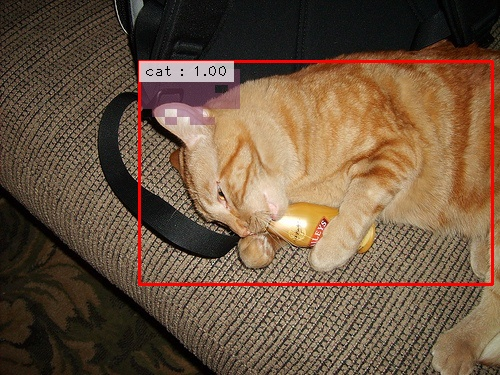
\includegraphics[width=\textwidth]{figures/samples/mask_pred_1.jpg}
        \caption{Pred: cat + mask}
    \end{subfigure}
    \hfill
    \begin{subfigure}[t]{0.235\textwidth}
        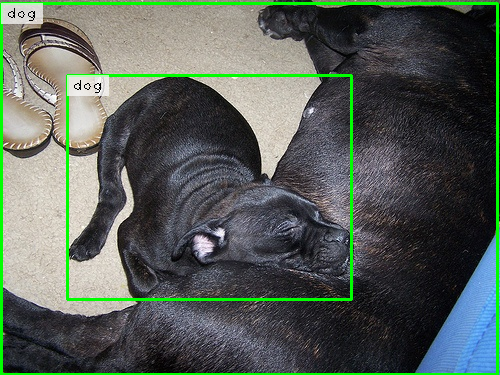
\includegraphics[width=\textwidth]{figures/samples/mask_gt_7.png}
        \caption{GT: dog (×2)}
    \end{subfigure}
    \hfill
    \begin{subfigure}[t]{0.235\textwidth}
        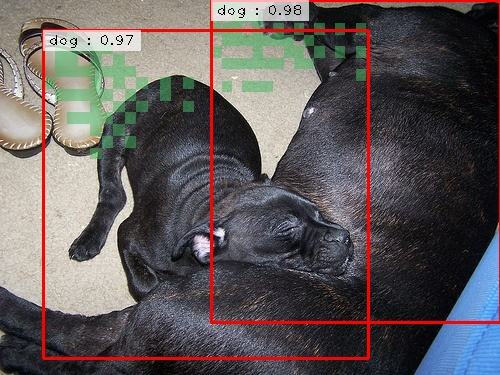
\includegraphics[width=\textwidth]{figures/samples/mask_pred_7.jpg}
        \caption{Pred: dog + masks}
    \end{subfigure}
    \caption{Instance segmentation results. Colored overlays show predicted binary masks for each detected object.}
    \label{fig:masks}
\end{figure}

% -----------------------------------------------------------------------
\section{Challenges and Solutions}

\paragraph{Anchor generation.} The stride has to be computed from the actual image/feature-map size ratio rather than assumed to be 16 everywhere, since resized images aren't always exact multiples of 16. Anchor centers also need to be offset by $\text{stride}/2$ to sit in the middle of each grid cell.

\paragraph{Proposal filtering order.} Clamping proposals to the image boundary can itself create degenerate boxes (zero width or height), so degenerate-box removal must come \emph{after} clamping, not before.

\paragraph{Class-specific regression.} The detection head predicts $21 \times 4$ deltas. During training, only the deltas for the GT class are supervised; at inference, only the top-scoring class's deltas are decoded. Getting the index slicing right---\texttt{box\_preds[range(N), labels]}---took some care.

\paragraph{Mask target generation.} To produce $28 \times 28$ GT masks aligned with the proposal, we crop the full-resolution GT mask to the GT bounding box and resize using RoI Align at spatial scale 1.0 (treating the crop as a $1 \times 1$ ``image''). Naive bilinear resize would not respect the box boundary.

\paragraph{VOC segmentation matching.} The integer instance indices in the \texttt{SegmentationObject} PNGs correspond to annotation order in the XML (1-indexed). A few images have edge cases where this correspondence breaks; a fallback using bounding box overlap handles those.

\paragraph{RoI Align gradient on MPS.} During local development on Apple MPS, RoI Align from torchvision occasionally hits device-specific issues. The final training ran on Colab CUDA where everything works cleanly, but supporting both backends in the code required checking that all ops have MPS-compatible implementations in the installed PyTorch version.

% -----------------------------------------------------------------------
\section{Conclusion}

Both Faster R-CNN and Mask R-CNN were implemented from scratch in PyTorch and trained on Pascal VOC 2007. The Faster R-CNN achieves 59.34\% mAP, consistent with what you'd expect from a VGG16 single-scale model. The Mask R-CNN extension matches that detection performance at 59.62\% mAP while additionally producing per-instance binary masks. The main bottleneck relative to stronger baselines is the backbone---switching to ResNet-50 with FPN would likely close most of the gap to the \textasciitilde70\% reference number.

% -----------------------------------------------------------------------
\bibliographystyle{plain}
\begin{thebibliography}{9}

\bibitem{ren2015faster}
S.\ Ren, K.\ He, R.\ Girshick, J.\ Sun.
\textit{Faster R-CNN: Towards Real-Time Object Detection with Region Proposal Networks}.
NeurIPS 2015.

\bibitem{he2017mask}
K.\ He, G.\ Gkioxari, P.\ Dollar, R.\ Girshick.
\textit{Mask R-CNN}.
ICCV 2017.

\bibitem{simonyan2014vgg}
K.\ Simonyan, A.\ Zisserman.
\textit{Very Deep Convolutional Networks for Large-Scale Image Recognition}.
ICLR 2015.

\bibitem{pascal2010}
M.\ Everingham et al.
\textit{The Pascal Visual Object Classes (VOC) Challenge}.
IJCV 2010.

\end{thebibliography}

\end{document}
